%#! platex ProgrammersGuideJa
\chapter{OpenFOAMの使用例}
\label{chap:3}
この章では,OpenFOAMディストリビューションと一緒に提供されている
様々なテストケースについて説明します.
その意図は,\href{UserGuideJa.pdf#chapter.2}{ユーザガイドの第2章}の
チュートリアルにあるものも含めて,あらゆる標準的なソルバに対する例題を提供することです.
これらの例題は,OpenFOAMのいくつかのツールや特徴,例えば内部の前・後処理,数値スキーム,
アルゴリズム,を紹介するように作られています.
また,主目的ではありませんが,これらはソルバの検証の意味ももっています.

それぞれの例題では,問題,形状,初期条件・境界条件の説明,
解くべき方程式,使われているモデル,そして必要な物性値の簡潔な説明をします.
例えば対称面を使ったりする場合は,解析領域は本来の形状の一部となるように選びます.
メッシュ生成の方法も説明しますが,たいてい\OFtool{blockMesh}を使います.
もちろん全ての例題にはメッシュを記述するファイルを含んだ
\OFpath{polyMesh}ディレクトリも一緒にありますので,
ユーザは簡単にメッシュを見ることができます.

例題は,インストールしたOpenFOAMの
\index{tutorialsディレクトリ@\OFpath{tutorials}ディレクトリ}%
\OFpath{tutorials}サブディレクトリ
の中にあるチュートリアルと対応しています.
それらはソルバごとのサブディレクトリにまとめられています.
例えば\OFtool{icoFoam}の全てのケースは\OFpath{icoFoam}サブディレクトリの中にあります.
例題を実行する前に,ユーザは自分のユーザ・アカウントの下にコピーしたほうがいいでしょう.
OpenFOAMの全てのケースを一つのディレクトリの下に保存しておくこと,
チュートリアルは\OFpath{\$FOAM\_RUN}ディレクトリの中にコピーすることをお薦めします.
もしユーザのアカウントの下にまだこのディレクトリが作られていなければ,
以下のように作ることができます.
\begin{OFverbatim}[terminal]
mkdir -p $FOAM_RUN
\end{OFverbatim}%$
以下のようにすれば,このディレクトリにチュートリアルをコピーできます.
\begin{OFverbatim}[terminal]
cp -r $FOAM_TUTORIALS/* $FOAM_RUN
\end{OFverbatim}



\section{円柱まわりの流れ}
\label{sec:3.1}
この例題では,\OFtool{potentialFoam}を使って
\index{えんちゅう@円柱!まわりのながれ@まわりの流れ}%
\index{えんちゅうまわりのながれ@円柱まわりの流れ}%
\index{れいだい@例題!えんちゅうまわりのながれ@円柱まわりの流れ}%
円柱まわりのポテンシャル流れを調べます.
この例題にはOpenFOAMの以下のような特徴を紹介します.
\begin{itemize}
\index{メッシュ!ひちょっこう@非直交}%
\index{ひちょっこうメッシュ@非直交メッシュ}%
 \item 非直交メッシュ
 \item OpenFOAMの問題に対する
\index{かいせきかい@解析解}%
解析解の生成
\end{itemize}


\subsection{問題設定}
\label{ssec:3.1.1}
この問題は以下のように定義されます.
\begin{description}
 \item[解析領域] \autoref{fig:3.1}に示すように,領域は2次元で,正方形領域と,
            その正方形の中心に配置された円柱からなります.


\begin{figure}[ht]
 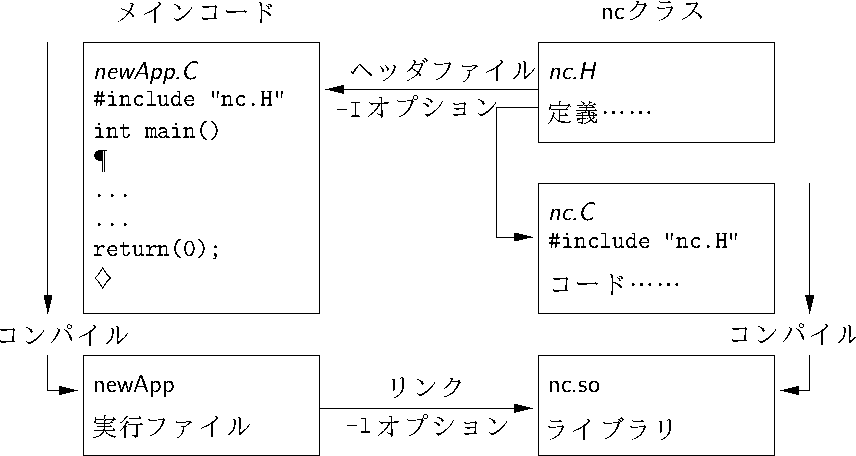
\includegraphics{fig-3-1}
 \caption{円柱まわり流れの配置}
 \label{fig:3.1}
\end{figure}


 \item[支配方程式] \mbox{}
            \begin{itemize}
             \item 非圧縮性流体の質量保存則
                   \begin{align}
                    \label{eq:3.1}
                    \nabla \inProd \bm{U} = 0
                   \end{align}
             \item 定常状態とみなした,非圧縮性,回転なしの流体の圧力方程式
                   \begin{align}
                    \label{eq:3.2}
                    \Laplacian p = 0
                   \end{align}
            \end{itemize}
 \item[境界条件] \mbox{}
            \begin{itemize}
             \item 入口(左)は速度固定$\bm{U} = (1,\ 0,\ 0) \unit{m/s}$
             \item 出口(右)は圧力固定$p = 0 \unit{Pa}$
             \item 滑りなし壁面(下)
             \item 対称面(上)
            \end{itemize}
 \item[初期条件] $U = 0 \unit{m/s}$,$p = 0 \unit{Pa}$\jdash
            これらはOpenFOAM入力ファイルで必要とされますが,
            この問題は定常状態なので解には必要ではありません.
\index{potentialFoamソルバ@\OFtool{potentialFoam}ソルバ}%
\index{ソルバ!potentialFoam@\OFtool{potentialFoam}}%
 \item[ソルバ名] \OFtool{potentialFoam}: ポテンシャル流れのコード,
            すなわち,流れが非圧縮性,定常,回転なし,非粘性とみなし,重力は無視します.
 \item[ケース名] \OFpath{\$FOAM\_TUTORIALS/potentialFoam}%
\footnote{訳注:これは古いバージョンでの配置.
現行バージョンでは\OFpath{\$FOAM\_TUTORIALS/basic/potentialFoam}にある.}%
            ディレクトリの中にある\OFcase{cylinder}ケース.
\end{description}


\subsection{\OFtool{potentialFoam}について}
\label{ssec:3.1.2}
ポテンシャル流れを仮定すると,比較的シンプルな形状の問題では解析解が存在するため,
\OFtool{potentialFoam}はOpenFOAMを検証するのに便利なソルバです.
この円柱まわり流れの例題には,数値解と比較できる解析解が存在します.
\OFtool{potentialFoam}は,問題に対して(適度に)保存されている初期$\bm{U}$場を
生成するユーティリティとしても利用することができます.
ケースによっては,初期場が不安定であることによる不安定さを避けるのに役立ちます.
端的にいえば,\OFtool{potentialFoam}はユーザが与えた非保存の初期場から,
保存された場を作りだします.


\subsection{メッシュ生成}
\label{ssec:3.1.3}
%% 原文の索引では solver に分類されているが,
%% それではおかしいので日本語版ではユーティリティとする.
\index{blockMesh@\OFtool{blockMesh}!ユーティリティ}%
\index{ユーティリティ!blockMesh@\OFtool{blockMesh}}%
\OFtool{blockMesh}を使ったメッシュ生成はユーザガイドで解説されています.
このケースでは,メッシュは\autoref{fig:3.2}に示すように10ブロックからなっています.
OpenFOAMでは全てのメッシュが3次元で扱われることを思い出してください.
2次元の問題を解きたければ,解かない3番目の方向に1セルのみをもつような
3次元メッシュを定義しなければなりません.
\autoref{fig:3.2}では,$z = -0.5$に沿った背面のみを示しており,
この中にある頂点番号は0〜18です.
それ以外の19個の頂点は,$z = +0.5$の正面にあり,
以下のメッシュ定義ファイルに示すように,
背面と同じ順番で番号付けられています.


\begin{figure}[b]
 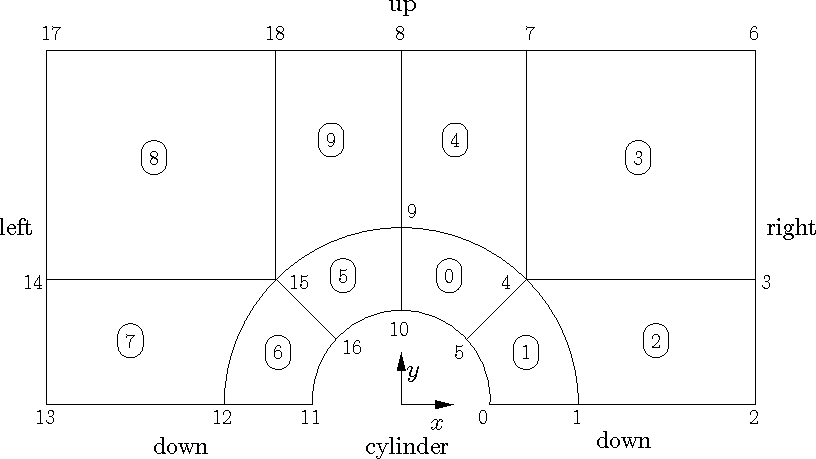
\includegraphics{fig-3-2}
 \caption{円柱形状のメッシュ}
 \label{fig:3.2}
\end{figure}


\begin{OFverbatim}[file, linenum]
/*--------------------------------*- C++ -*----------------------------------*\
| =========                 |                                                 |
| \\      /  F ield         | OpenFOAM: The Open Source CFD Toolbox           |
|  \\    /   O peration     | Version:  2.2.0                                 |
|   \\  /    A nd           | Web:      www.OpenFOAM.org                      |
|    \\/     M anipulation  |                                                 |
\*---------------------------------------------------------------------------*/
FoamFile
{
    version     2.0;
    format      ascii;
    class       dictionary;
    object      blockMeshDict;
}
// * * * * * * * * * * * * * * * * * * * * * * * * * * * * * * * * * * * * * //

convertToMeters 1;

vertices #codeStream
{
    codeInclude
    #{
        #include "pointField.H"
    #};

    code
    #{
        pointField points(19);
        points[0]  = point(0.5, 0, -0.5);
        points[1]  = point(1, 0, -0.5);
        points[2]  = point(2, 0, -0.5);
        points[3]  = point(2, 0.707107, -0.5);
        points[4]  = point(0.707107, 0.707107, -0.5);
        points[5]  = point(0.353553, 0.353553, -0.5);
        points[6]  = point(2, 2, -0.5);
        points[7]  = point(0.707107, 2, -0.5);
        points[8]  = point(0, 2, -0.5);
        points[9]  = point(0, 1, -0.5);
        points[10] = point(0, 0.5, -0.5);
        points[11] = point(-0.5, 0, -0.5);
        points[12] = point(-1, 0, -0.5);
        points[13] = point(-2, 0, -0.5);
        points[14] = point(-2, 0.707107, -0.5);
        points[15] = point(-0.707107, 0.707107, -0.5);
        points[16] = point(-0.353553, 0.353553, -0.5);
        points[17] = point(-2, 2, -0.5);
        points[18] = point(-0.707107, 2, -0.5);

        // Duplicate z points
        label sz = points.size();
        points.setSize(2*sz);
        for (label i = 0; i < sz; i++)
        {
            const point& pt = points[i];
            points[i+sz] = point(pt.x(), pt.y(), -pt.z());
        }

        os  << points;
    #};
};


blocks          
(
    hex (5 4 9 10 24 23 28 29) (10 10 1) simpleGrading (1 1 1)
    hex (0 1 4 5 19 20 23 24) (10 10 1) simpleGrading (1 1 1)
    hex (1 2 3 4 20 21 22 23) (20 10 1) simpleGrading (1 1 1)
    hex (4 3 6 7 23 22 25 26) (20 20 1) simpleGrading (1 1 1)
    hex (9 4 7 8 28 23 26 27) (10 20 1) simpleGrading (1 1 1)
    hex (15 16 10 9 34 35 29 28) (10 10 1) simpleGrading (1 1 1)
    hex (12 11 16 15 31 30 35 34) (10 10 1) simpleGrading (1 1 1)
    hex (13 12 15 14 32 31 34 33) (20 10 1) simpleGrading (1 1 1)
    hex (14 15 18 17 33 34 37 36) (20 20 1) simpleGrading (1 1 1)
    hex (15 9 8 18 34 28 27 37) (10 20 1) simpleGrading (1 1 1)
);

edges           
(
    arc 0 5 (0.469846 0.17101 -0.5)
    arc 5 10 (0.17101 0.469846 -0.5)
    arc 1 4 (0.939693 0.34202 -0.5)
    arc 4 9 (0.34202 0.939693 -0.5)
    arc 19 24 (0.469846 0.17101 0.5)
    arc 24 29 (0.17101 0.469846 0.5)
    arc 20 23 (0.939693 0.34202 0.5)
    arc 23 28 (0.34202 0.939693 0.5)
    arc 11 16 (-0.469846 0.17101 -0.5)
    arc 16 10 (-0.17101 0.469846 -0.5)
    arc 12 15 (-0.939693 0.34202 -0.5)
    arc 15 9 (-0.34202 0.939693 -0.5)
    arc 30 35 (-0.469846 0.17101 0.5)
    arc 35 29 (-0.17101 0.469846 0.5)
    arc 31 34 (-0.939693 0.34202 0.5)
    arc 34 28 (-0.34202 0.939693 0.5)
);

boundary
(
    down
    {
        type symmetryPlane;
        faces
        (
            (0 1 20 19)
            (1 2 21 20)
            (12 11 30 31)
            (13 12 31 32)
        );
    }
    right
    {
        type patch;
        faces
        (
            (2 3 22 21)
            (3 6 25 22)
        );
    }
    up
    {
        type symmetryPlane;
        faces
        (
            (7 8 27 26)
            (6 7 26 25)
            (8 18 37 27)
            (18 17 36 37)
        );
    }
    left
    {
        type patch;
        faces
        (
            (14 13 32 33)
            (17 14 33 36)
        );
    }
    cylinder
    {
        type symmetryPlane;
        faces
        (
            (10 5 24 29)
            (5 0 19 24)
            (16 10 29 35)
            (11 16 35 30)
        );
    }
);

mergePatchPairs
(
);

// ************************************************************************* //
\end{OFverbatim}

\subsection{境界条件と初期条件}
\label{ssec:3.1.4}
\OFtool{FoamX}を使うか,ケース・ファイルを手で編集して,
\autoref{fig:3.1}に示す問題に合致するように境界条件を設定します.
つまり,左側の境界は\OFboundary{Inlet},
右側の境界は\OFboundary{Outlet},
そして下側と円柱の境界は\OFboundary{symmetryPlane}となります.
上側の境界条件は,
$y$方向に無限の領域を仮定して得られた解析解に対して,
最もよく比較できるように選択します.
結果として,この境界に一致する面上においては,
法線方向の$\bm{U}$の勾配は小さくなります.
したがって,法線成分がゼロとなるような条件を採用します.
つまり,\OFboundary{symmetryPlane}を設定し,
これによって解析解と適切な比較ができるようにします.


\subsection{ケースの実行}
\label{ssec:3.1.5}
この問題では,流れは非圧縮性で非粘性を仮定しているので,
流体の物性値は何も指定する必要がありません.
\index{ディレクトリ!system@\OFpath{system}}%
\index{systemディレクトリ@\OFpath{system}ディレクトリ}%
\OFpath{system}サブディレクトリの中の,
\OFdictionary{controlDict}に実行のための制御パラメータを指定します.
定常流れを仮定しているため,1ステップだけ実行すればよいことに注意してください.
\begin{OFverbatim}[file, linenum]
/*--------------------------------*- C++ -*----------------------------------*\
| =========                 |                                                 |
| \\      /  F ield         | OpenFOAM: The Open Source CFD Toolbox           |
|  \\    /   O peration     | Version:  2.2.0                                 |
|   \\  /    A nd           | Web:      www.OpenFOAM.org                      |
|    \\/     M anipulation  |                                                 |
\*---------------------------------------------------------------------------*/
FoamFile
{
    version     2.0;
    format      ascii;
    class       dictionary;
    location    "system";
    object      controlDict;
}
// * * * * * * * * * * * * * * * * * * * * * * * * * * * * * * * * * * * * * //

application     potentialFoam;

startFrom       startTime;

startTime       0;

stopAt          endTime;

endTime         1;

deltaT          1;

writeControl    timeStep;

writeInterval   1;

purgeWrite      0;

writeFormat     ascii;

writePrecision  6;

writeCompression off;

timeFormat      general;

timePrecision   6;

runTimeModifiable true;

functions
{
    difference
    {
        // Load the library containing the 'coded' functionObject
        functionObjectLibs ("libutilityFunctionObjects.so");
        type coded;
        // Name of on-the-fly generated functionObject
        redirectType error;
        code
        #{
            // Lookup U
            Info<< "Looking up field U\n" << endl;
            const volVectorField& U = mesh().lookupObject<volVectorField>("U");

            Info<< "Reading inlet velocity  uInfX\n" << endl;

            scalar ULeft = 0.0;
            label leftI = mesh().boundaryMesh().findPatchID("left");
            const fvPatchVectorField& fvp = U.boundaryField()[leftI];
            if (fvp.size())
            {
                ULeft = fvp[0].x();
            }
            reduce(ULeft, maxOp<scalar>());

            dimensionedScalar uInfX
            (
                "uInfx",
                dimensionSet(0, 1, -1, 0, 0),
                ULeft
            );

            Info << "U at inlet = " << uInfX.value() << " m/s" << endl;


            scalar magCylinder = 0.0;
            label cylI = mesh().boundaryMesh().findPatchID("cylinder");
            const fvPatchVectorField& cylFvp = mesh().C().boundaryField()[cylI];
            if (cylFvp.size())
            {
                magCylinder = mag(cylFvp[0]);
            }
            reduce(magCylinder, maxOp<scalar>());

            dimensionedScalar radius
            (
                "radius",
                dimensionSet(0, 1, 0, 0, 0),
                magCylinder
            );

            Info << "Cylinder radius = " << radius.value() << " m" << endl;

            volVectorField UA
            (
                IOobject
                (
                    "UA",
                    mesh().time().timeName(),
                    U.mesh(),
                    IOobject::NO_READ,
                    IOobject::AUTO_WRITE
                ),
                U
            );

            Info<< "\nEvaluating analytical solution" << endl;

            const volVectorField& centres = UA.mesh().C();
            volScalarField magCentres(mag(centres));
            volScalarField theta(acos((centres & vector(1,0,0))/magCentres));

            volVectorField cs2theta
            (
                cos(2*theta)*vector(1,0,0)
              + sin(2*theta)*vector(0,1,0)
            );

            UA = uInfX*(dimensionedVector(vector(1,0,0))
              - pow((radius/magCentres),2)*cs2theta);

            // Force writing of UA (since time has not changed)
            UA.write();

            volScalarField error("error", mag(U-UA)/mag(UA));

            Info<<"Writing relative error in U to " << error.objectPath()
                << endl;

            error.write();
        #};
    }
}


// ************************************************************************* //
\end{OFverbatim}
\OFtool{potentialFoam}は,
圧力の方程式について反復計算を行い,
反復が成功すればラプラシアン項の非直交補正に合致する陽的な項が更新されます.
圧力の方程式についての反復計算の回数は,\OFdictionary{controlDict}の中の
\OFkeyword{nNonOrthogonalCorrectors}キーワードで制御します.
一つの例として,\OFkeyword{nNonOrthogonalCorrectors}を0に設定すれば,反復は行われません.
つまり,圧力の方程式が1回だけ解かれ,非直交補正は行われません.
その解を\autoref{fig:3.3} (a) に示します(定常状態の解析が完了した$t = 1$において).
\autoref{fig:3.3} (c) に示す解析解のように,
領域を横切るなめらかな流線となる解を期待しているのですが,
例えば,ブロック0,1,そして3の交点のように,
メッシュの非直交性が強い領域において,明らかな誤差があります.
\OFkeyword{nNonOrthogonalCorrectors}を3に設定し,
非直交補正を加えて再度ケースを実行してみましょう.
\autoref{fig:3.3} (b) のように,
解はなめらかな流線となり,非直交性に起因する顕著な誤差はありません.


\begin{figure}[p]
 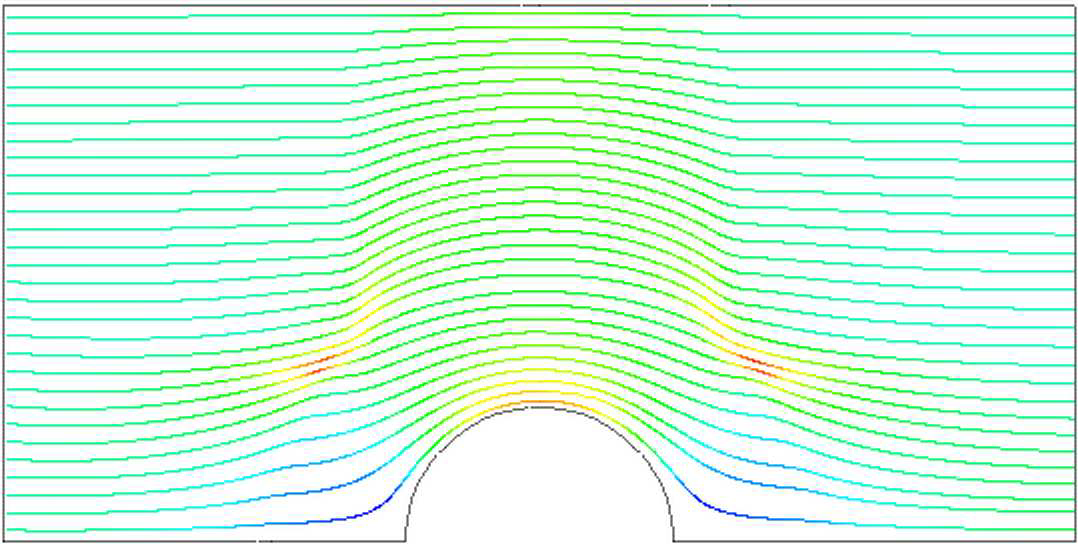
\includegraphics[scale=0.36]{fig-3-3-a}\par
 \medskip
 (a) 非直交補正なし\par
 \bigskip
 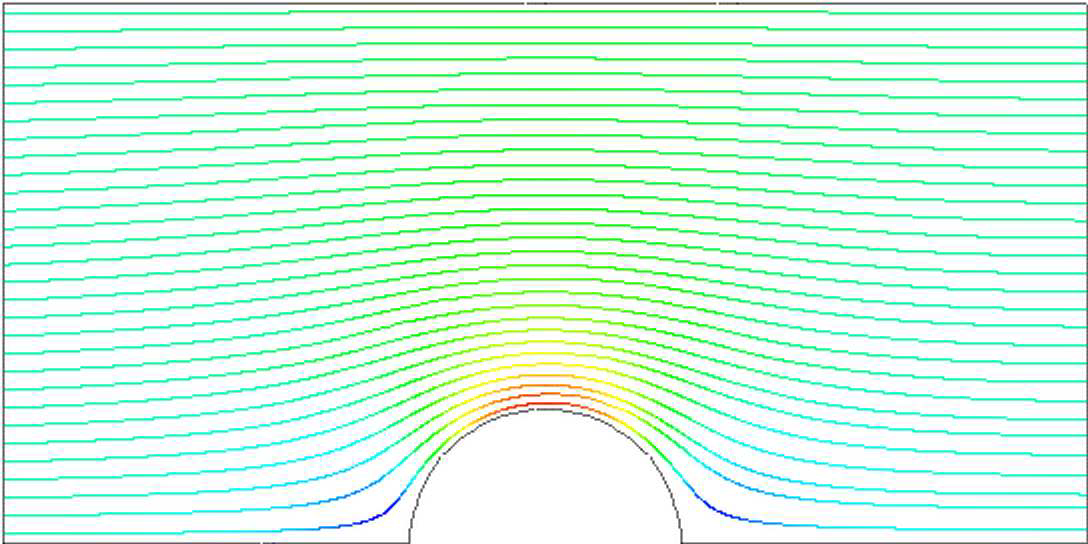
\includegraphics[scale=0.36]{fig-3-3-b}\par
 \medskip
 (b) 非直交補正あり\par
 \bigskip
 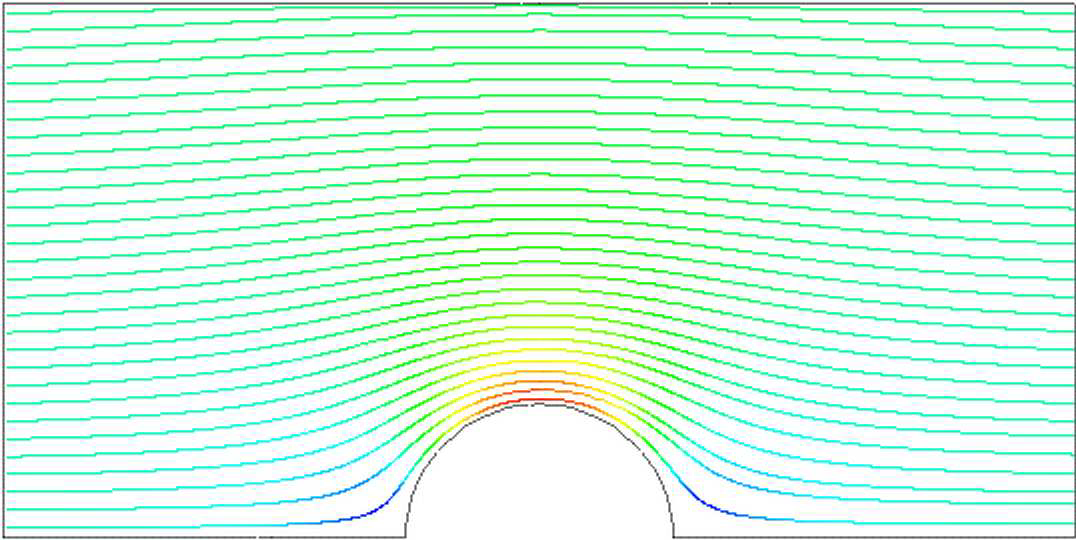
\includegraphics[scale=0.36]{fig-3-3-c}\par
 \medskip
 (c) 解析解\par
 \medskip
 \caption{ポテンシャル流れの流線}
 \label{fig:3.3}
\end{figure}


% \subsection{解析解の作成}
% \label{ssec:3.1.6}
% このポテンシャル流れのケースに対する解析解を作成するためのソースコードが
% \OFpath{\$FOAM\_TUTORIALS/basic/potentialFoam/cylinder/analyticalCylinder}ディレクトリにあります.
% 円柱の中心から距離$d$で角度$\theta$の点における速度は,解析的に以下のように記述されます.
% \begin{align}
%  \label{eq:3.3}
%  U_{x} &= U_{\infty}\left[1 - \left(\frac{r}{d}\right)^{2}\cos2\theta\right] &
%  U_{y} &= U_{\infty}\left(\frac{r}{d}\right)^{2}\sin2\theta
% \end{align}
% ここで,$r$は円柱の半径,$U_{\infty}$は流入速度です.
% $\theta$は$x$軸からの角度を表しています.

% \OFpath{analyticalCylinder}ディレクトリの中にあるソースコードについて,少し詳しく説明しましょう.
% \OFpath{createFields.H}の中では,
% \OFtool{analyticalCylinder}の実行中に場のデータが上書きされないように
% \texttt{IOobject::NO\_WRITE}オプションを使って,速度場が読み込まれます.
% メッシュから読み込まれたデータから入口速度と円柱の半径が取り出され,
% 解析解を保存するための場\OFkeyword{UA}が用意されます.
% \begin{OFverbatim}[file, linenum]
% Info<< "Reading field U\n" << endl;
% volVectorField U
% (
%     IOobject
%     (
%         "U",
%         runTime.timeName(),
%         mesh,
%         IOobject::MUST_READ,
%         IOobject::NO_WRITE
%     ),
%     mesh
% );

% Info<< "Reading inlet velocity  uInfX\n" << endl;

% dimensionedScalar uInfX
% (
%     "uInfx",
%     dimensionSet(0, 1, -1, 0, 0),
%     U.boundaryField()[3][0].x()
% );
% Info << "U at inlet = " << uInfX.value() << " m/s" << endl;

% dimensionedScalar radius
% (
%     "radius",
%     dimensionSet(0, 1, 0, 0, 0),
%     mag(U.mesh().boundary()[4].Cf()[0])
% );

% Info << "Cylinder radius = " << radius.value() << " m" << endl;

% volVectorField UA
% (
%     IOobject
%     (
%         "UA",
%         runTime.timeName(),
%         mesh,
%         IOobject::NO_READ,
%         IOobject::AUTO_WRITE
%     ),
%     U
% );
% \end{OFverbatim}
% メインのコード\OFpath{analyticalCylinder.C}は,以下のタスクを実行します.
% \begin{itemize}
%  \item \texttt{runTime++}で時間ステップを進める.
% \OFrevision{\texttt{runTime++}なんて登場しない??}
%  \item テンソル計算により\OFkeyword{UA}の解析解を生成する.
%  \item \texttt{runTime.writeObjects()}で解をファイルに書きだす.
% \end{itemize}
% \begin{OFverbatim}[file, linenum]
% /*---------------------------------------------------------------------------*\
%   =========                 |
%   \\      /  F ield         | OpenFOAM: The Open Source CFD Toolbox
%    \\    /   O peration     |
%     \\  /    A nd           | Copyright (C) 1991-2010 OpenCFD Ltd.
%      \\/     M anipulation  |
% -------------------------------------------------------------------------------
% License
%     This file is part of OpenFOAM.

%     OpenFOAM is free software: you can redistribute it and/or modify it
%     under the terms of the GNU General Public License as published by
%     the Free Software Foundation, either version 3 of the License, or
%     (at your option) any later version.

%     OpenFOAM is distributed in the hope that it will be useful, but WITHOUT
%     ANY WARRANTY; without even the implied warranty of MERCHANTABILITY or
%     FITNESS FOR A PARTICULAR PURPOSE.  See the GNU General Public License
%     for more details.

%     You should have received a copy of the GNU General Public License
%     along with OpenFOAM.  If not, see <http://www.gnu.org/licenses/>.

% Application
%     analyticalCylinder

% Description
%     Generates an analytical solution for potential flow around a cylinder.
%     Can be compared with the solution from the potentialFlow/cylinder example.

% \*---------------------------------------------------------------------------*/

% #include "fvCFD.H"


% // * * * * * * * * * * * * * * * * * * * * * * * * * * * * * * * * * * * * * //

% int main(int argc, char *argv[])
% {

% #   include "setRootCase.H"

% #   include "createTime.H"
% #   include "createMesh.H"
% #   include "createFields.H"

% // * * * * * * * * * * * * * * * * * * * * * * * * * * * * * * * * * * * * * //

%     Info << "\nEvaluating analytical solution" << endl;

%     volVectorField centres = UA.mesh().C();
%     volScalarField magCentres = mag(centres);
%     volScalarField theta = acos((centres & vector(1,0,0))/magCentres);

%     volVectorField cs2theta =
%         cos(2*theta)*vector(1,0,0)
%       + sin(2*theta)*vector(0,1,0);

%     UA = uInfX*(dimensionedVector(vector(1,0,0))
%       - pow((radius/magCentres),2)*cs2theta);

%     // Force writing of UA (since time has not changed)
%     UA.write();

%     Info<< "end" << endl;

%     return 0;
% }

% // ************************************************************************* //
% \end{OFverbatim}
% このユーティリティは通常通り\OFtool{wmake}でコンパイルできるはずです.
% そして,以下のようにタイプして実行できます.
% \OFrevision{実行方法が古い.}
% \begin{OFverbatim}[terminal]
% analyticalCylinder $FOAM_RUN/potentialFoam cylinder
% \end{OFverbatim}%$
% 解析解は\autoref{fig:3.3} (c) のように流線でプロットできます.
% 解析解と数値解の上面における相違は,
% 解析解では無限境界を仮定しているのに対し,
% 数値解では\OFboundary{zeroGradient}境界条件を使用しているためです.


% \subsection{課題}
% \label{ssec:3.1.7}
% 数値解と\OFcase{analyticalCylinder}の解析解を何らかの手法を使って比較することで,
% 数値解の精度について調査してみましょう.


\section{バック・ステップ上の定常乱流}
\label{sec:3.2}
\index{バック・ステップじょうのながれ@バック・ステップ上の流れ}%
\index{れいだい@例題!バック・ステップじょうのながれ@バック・ステップ上の流れ}%
この例題では,後方に面する段差上を流れる
\index{らんりゅう@乱流!ていじょう@定常}%
定常乱流について調べます.
この問題設定は,PitzとDailyが実験的に調べたものに由来しており,
数値解との比較することができます.
この例題では,新たにOpenFOAMの以下のような特徴を紹介します.
\begin{itemize}
 \item 完全なメッシュの
\index{メッシュ!こうばい@勾配}%
 勾配付け機能を利用した,\OFtool{blockMesh}によるメッシュ生成
 \item 定常乱流
\end{itemize}


\subsection{問題設定}
\label{ssec:3.2.1}
問題は以下のように定義します.
\begin{description}
 \item[解析領域] 領域は2次元で,\autoref{fig:3.4}に示すように,
            短い入口,バック・ステップ,そして出口の先細ノズルからなります.


\begin{figure}[ht]
 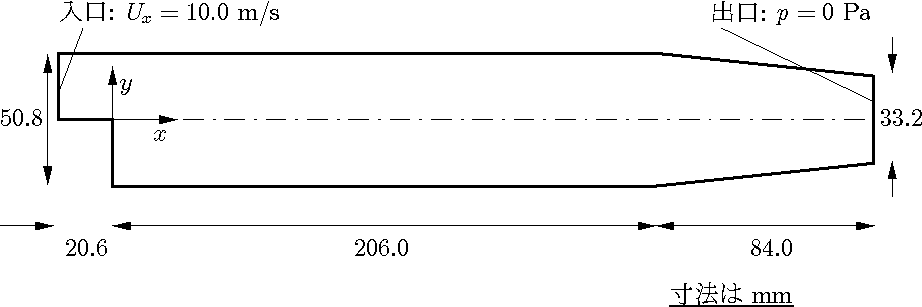
\includegraphics{fig-3-4}
 \caption{バック・ステップの計算領域形状}
 \label{fig:3.4}
\end{figure}


 \item[支配方程式] \mbox{}
            \begin{itemize}
             \item 非圧縮性流体の質量保存則
                   \begin{align}
                    \label{eq:3.3}
                    \nabla \inProd \bm{U} = 0
                   \end{align}
             \item 定常流れの運動量方程式
                   \begin{align}
                    \label{eq:3.4}
                    \nabla \inProd (\bm{U}\bm{U}) + \nabla \inProd \bm{R} = -\nabla p
                   \end{align}
                   ここで$p$は運動学的圧力であり,
                   \OFrevision{$p/\rho$のこと.もっと良い訳は?}%
                   (やや単純化しすぎですが)$\bm{R} = \nu_{\mathrm{eff}}\nabla\bm{U}$は
                   粘性応力の項で,実効動粘性係数$\nu_{\mathrm{eff}}$は
                   選択された輸送・乱流モデルで計算されます.
            \end{itemize}
 \item[初期条件] $U = 0 \unit{m/s}$,$p = 0 \unit{Pa}$\jdash
            これらはOpenFOAM入力ファイルで必要とされますが,
            この問題は定常状態なので解には必要ではありません.
 \item[境界条件] \mbox{}
            \begin{itemize}
             \item 入口(左)は速度固定$\bm{U} = (10,\ 0,\ 0) \unit{m/s}$
             \item 出口(右)は圧力固定$p = 0 \unit{Pa}$
             \item それ以外の境界は,滑りなし壁面
            \end{itemize}
 \item[輸送特性] \mbox{}
            \begin{itemize}
             \item 空気の動粘性係数
                   $\nu = \mu/\rho = 18.1 \times 10^{-6}/1.293 = 14.0 \unit{\micro m^{2}/s}$
            \end{itemize}
 \item[乱流モデル] \mbox{}
            \begin{itemize}
             \item 標準$k$--$\epsilon$
             \item 係数:$C_{\mu} = 0.09$; $C_{1} = 1.44$; $C_{2} = 1.92$;
                   $\alpha_{k} = 1$; $\alpha_{\epsilon} = 0.76923$.
            \end{itemize}
 \item[ソルバ名]
 \index{simpleFoamソルバ@\OFtool{simpleFoam}ソルバ}%
 \index{ソルバ!simpleFoam@\OFtool{simpleFoam}}%
 \OFtool{simpleFoam}: 定常非圧縮性流れ用.
 \item[ケース名] \OFpath{\$FOAM\_TUTORIALS/simpleFoam}%
\footnote{訳注:これは古いバージョンでの配置.
現行バージョンでは\OFpath{\$FOAM\_TUTORIALS/incompressible/simpleFoam}にある.}%
            ディレクトリの中にある\OFcase{pitzDaily}ケース.
\end{description}

この問題は\OFtool{simpleFoam}を使って解きます.
SIMPLEアルゴリズムを用いた定常流れのためのソルバなのでこのように名付けられています.
このソルバは,標準のOpenFOAMリリースの
\OFclass{incompressibleTurbulenceModels}
\index{incompressibleTurbulenceModels@\OFclass{incompressibleTurbulenceModels}!ライブラリ}%
\index{ライブラリ!incompressibleTurbulenceModels@\OFclass{incompressibleTurbulenceModels}}%
ライブラリの中の乱流モデル,
および\OFclass{incompressibleTransportModels}
\index{incompressibleTransportModels@\OFclass{incompressibleTransportModels}!ライブラリ}%
\index{ライブラリ!incompressibleTransportModels@\OFclass{incompressibleTransportModels}}%
ライブラリの中の非ニュートン流体モデル
の全てを適用することができます.


\subsection{メッシュ生成}
\label{ssec:3.2.2}
この問題の流れはちょうどよく複雑で,適切な解を得るにはメッシュの
\index{メッシュ!こうばい@勾配}%
勾配付けが必要となります.
一般に,最もせん断力のかかる領域が特に決め手であり,せん断力の小さい領域より細かいメッシュを必要とします.
どこで大きなせん断力が生じるかは,計算が進んだらどのような解になるはずであるかを考察することで予想できます.
入口では$x$方向の強い一様流ですが,段差を過ぎると,
下側の流体に対してせん断力を生じ,領域の下半分に渦を生じます.
したがって,せん断力の大きな領域は領域の中心線付近と壁付近となるでしょう.

領域は,\autoref{fig:3.5}に示すように12個のブロックに分割されます.


\begin{figure}[ht]
 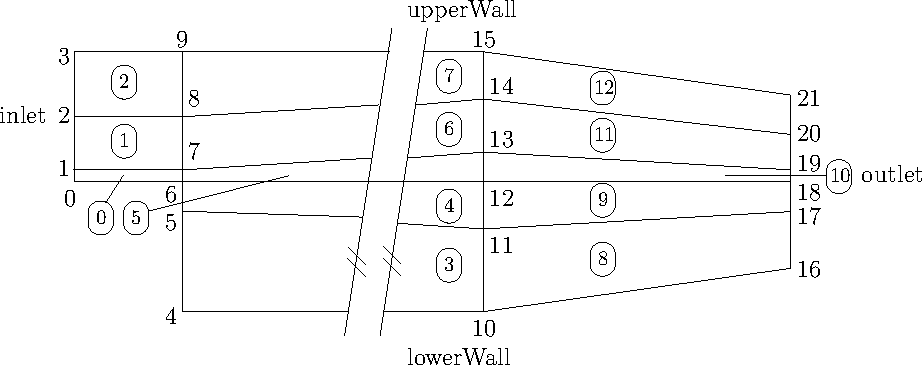
\includegraphics{fig-3-5}
 \caption{バック・ステップ問題のブロック分け}
 \label{fig:3.5}
\end{figure}


OpenFOAMではメッシュは常に3次元なので,\autoref{fig:3.5}では$z = -0.5$に沿った背面を示しています.
全ての頂点とブロックは,以下のメッシュ記述ファイルで与えられます.
\begin{OFverbatim}[file, linenum]
/*--------------------------------*- C++ -*----------------------------------*\
| =========                 |                                                 |
| \\      /  F ield         | OpenFOAM: The Open Source CFD Toolbox           |
|  \\    /   O peration     | Version:  2.2.0                                 |
|   \\  /    A nd           | Web:      www.OpenFOAM.org                      |
|    \\/     M anipulation  |                                                 |
\*---------------------------------------------------------------------------*/
FoamFile
{
    version     2.0;
    format      ascii;
    class       dictionary;
    object      blockMeshDict;
}
// * * * * * * * * * * * * * * * * * * * * * * * * * * * * * * * * * * * * * //

convertToMeters 0.001;

vertices
(
    (-20.6 0 -0.5)
    (-20.6 3 -0.5)
    (-20.6 12.7 -0.5)
    (-20.6 25.4 -0.5)
    (0 -25.4 -0.5)
    (0 -5 -0.5)
    (0 0 -0.5)
    (0 3 -0.5)
    (0 12.7 -0.5)
    (0 25.4 -0.5)
    (206 -25.4 -0.5)
    (206 -8.5 -0.5)
    (206 0 -0.5)
    (206 6.5 -0.5)
    (206 17 -0.5)
    (206 25.4 -0.5)
    (290 -16.6 -0.5)
    (290 -6.3 -0.5)
    (290 0 -0.5)
    (290 4.5 -0.5)
    (290 11 -0.5)
    (290 16.6 -0.5)
    (-20.6 0 0.5)
    (-20.6 3 0.5)
    (-20.6 12.7 0.5)
    (-20.6 25.4 0.5)
    (0 -25.4 0.5)
    (0 -5 0.5)
    (0 0 0.5)
    (0 3 0.5)
    (0 12.7 0.5)
    (0 25.4 0.5)
    (206 -25.4 0.5)
    (206 -8.5 0.5)
    (206 0 0.5)
    (206 6.5 0.5)
    (206 17 0.5)
    (206 25.4 0.5)
    (290 -16.6 0.5)
    (290 -6.3 0.5)
    (290 0 0.5)
    (290 4.5 0.5)
    (290 11 0.5)
    (290 16.6 0.5)
);

blocks
(
    hex (0 6 7 1 22 28 29 23) (18 7 1) simpleGrading (0.5 1.8 1)
    hex (1 7 8 2 23 29 30 24) (18 10 1) simpleGrading (0.5 4 1)
    hex (2 8 9 3 24 30 31 25) (18 13 1) simpleGrading (0.5 0.25 1)
    hex (4 10 11 5 26 32 33 27) (180 18 1) simpleGrading (4 1 1)
    hex (5 11 12 6 27 33 34 28) (180 9 1) edgeGrading (4 4 4 4 0.5 1 1 0.5 1 1 1 1)
    hex (6 12 13 7 28 34 35 29) (180 7 1) edgeGrading (4 4 4 4 1.8 1 1 1.8 1 1 1 1)
    hex (7 13 14 8 29 35 36 30) (180 10 1) edgeGrading (4 4 4 4 4 1 1 4 1 1 1 1)
    hex (8 14 15 9 30 36 37 31) (180 13 1) simpleGrading (4 0.25 1)
    hex (10 16 17 11 32 38 39 33) (25 18 1) simpleGrading (2.5 1 1)
    hex (11 17 18 12 33 39 40 34) (25 9 1) simpleGrading (2.5 1 1)
    hex (12 18 19 13 34 40 41 35) (25 7 1) simpleGrading (2.5 1 1)
    hex (13 19 20 14 35 41 42 36) (25 10 1) simpleGrading (2.5 1 1)
    hex (14 20 21 15 36 42 43 37) (25 13 1) simpleGrading (2.5 0.25 1)
);

edges
(
);

boundary
(
    inlet
    {
        type patch;
        faces
        (
            (0 22 23 1)
            (1 23 24 2)
            (2 24 25 3)
        );
    }
    outlet
    {
        type patch;
        faces
        (
            (16 17 39 38)
            (17 18 40 39)
            (18 19 41 40)
            (19 20 42 41)
            (20 21 43 42)
        );
    }
    upperWall
    {
        type wall;
        faces
        (
            (3 25 31 9)
            (9 31 37 15)
            (15 37 43 21)
        );
    }
    lowerWall
    {
        type wall;
        faces
        (
            (0 6 28 22)
            (6 5 27 28)
            (5 4 26 27)
            (4 10 32 26)
            (10 16 38 32)
        );
    }
    frontAndBack
    {
        type empty;
        faces
        (
            (22 28 29 23)
            (23 29 30 24)
            (24 30 31 25)
            (26 32 33 27)
            (27 33 34 28)
            (28 34 35 29)
            (29 35 36 30)
            (30 36 37 31)
            (32 38 39 33)
            (33 39 40 34)
            (34 40 41 35)
            (35 41 42 36)
            (36 42 43 37)
            (0 1 7 6)
            (1 2 8 7)
            (2 3 9 8)
            (4 5 11 10)
            (5 6 12 11)
            (6 7 13 12)
            (7 8 14 13)
            (8 9 15 14)
            (10 11 17 16)
            (11 12 18 17)
            (12 13 19 18)
            (13 14 20 19)
            (14 15 21 20)
        );
    }
);

mergePatchPairs
(
);

// ************************************************************************* //
\end{OFverbatim}
この問題の最大の特徴は,
\href{UserGuideJa.pdf#subsection.5.3.1}{ユーザガイドの5.3.1項}で
述べた\OFtool{blockMesh}の完全なメッシュの勾配付けの機能を使っていることです.
ブロック4,5および6では,12個の拡大率からなる完全なリストを使っていることがわかります.
これらの拡大率は,それぞれのブロックの線分について,
最初の四つは局所的な$x_{1}$方向に沿った線分,
次の四つは局所的な$x_{2}$方向の線分,最後の四つは局所的な$x_{3}$方向の線分に対応しています.
ブロック4,5および6では,局所的な$x_{1}$および$x_{2}$方向の線分すべてに対して
等しい比率となっていますが,$x_{2}$方向については違います.
これは全てのブロックで,大域座標の$y$に対応しています.
\href{UserGuideJa.pdf#subsection.5.3.1}{ユーザガイドの5.3.1項}で
述べたブロック定義と関連付けて使われている比率を考えると,
\autoref{fig:3.5}のブロック4,5および6において,
左側と右側の線分に沿って,異なった勾配付けが規定されていることがわかります.
この異なる勾配付けの目的は,流れの最も重大な領域である,
段差で流れが曲がるところにおいて細かいメッシュを生成し,
それ以外の領域にかけて拡大していくようにするためです.

コマンドラインまたは\OFtool{FoamX}から\OFtool{blockMesh}を使ってメッシュを生成し,
先に例示したように可視化します.


\subsection{境界条件と初期条件}
\label{ssec:3.2.3}
ケースのファイルは,\OFtool{FoamX}の中で,または手作業で閲覧・編集できます.
このケースでは,速度$\bm{U}$,圧力$p$,
乱流の運動エネルギ$k$および散逸率$\varepsilon$について,
初期および境界の場を設定する必要があります.
境界条件は,\OFtool{FoamX}で物理的なパッチのタイプを設定することで指定できます.
上下の壁は\OFkeyword{Wall},左側のパッチは\OFkeyword{Inlet},
そして右側のパッチは\OFkeyword{Outlet}に設定します.
入口の$\bm{U}$,$k$および$\varepsilon$については,
物理境界条件として\OFboundary{fixedValue}を指定する必要があります.
$\bm{U}$は問題設定により与えられていますが,
$k$と$\varepsilon$については
\href{UserGuideJa.pdf#subsubsection.2.1.8.1}{ユーザガイドの2.1.8.1}で
述べたのと同様な方法で,ユーザが決めなければなりません.
入口においては,乱流は等方性であり,変動は$\bm{U}$の$5\unit{\%}$と仮定します.
\begin{align}
 \label{eq:3.5}
 U'_{x} = U'_{y} = U'_{z} = \frac{5}{100}10 = 0.5 \unit{m/s}
\end{align}
および
\begin{align}
 \label{eq:3.6}
 k = \frac{3}{2}(0.5)^{2} = 0.375 \unit{m^{2}/s^{3}}
\end{align}
が得られます.
乱流の長さスケール$l$を入口幅の$10\unit{\%}$と見積もれば,
\begin{align}
 \label{eq:3.7}
 \varepsilon = \frac{C_{\mu}^{0.75}k^{1.5}}{l}
 = \frac{0.09^{0.75} \times 0.375^{1.5}}{0.1 \times 25.4 \times 10^{-3}}
 = 14.855 \unit{m^{2}/s^{3}}
\end{align}
となります.
出口においては,圧力$p = 0 \unit{Pa}$だけしか指定する必要はありません.


\subsection{ケースの制御}
\label{ssec:3.2.4}
\OFdictionary{fvSchemes}の選択は以下のようにします.
\OFkeyword{timeScheme}は\OFkeyword{steadyState}とし,
\OFkeyword{gradScheme}および\OFkeyword{laplacianScheme}は
デフォルトとして\OFkeyword{Gauss}を設定します.
また,有界性を保証するため\OFkeyword{divScheme}は\OFkeyword{UD}とします.

\OFdictionary{fvTolerances}の設定には特に注意を払う必要があります.%
\footnote{訳注:この段落は古いバージョン向けの説明となっている.
現行バージョンでは\OFdictionary{fvTolerances}ではなく\OFdictionary{fvSolution},
\OFkeyword{solverTolerance}ではなく\OFkeyword{tolerance},
\OFkeyword{solverRelativeTolerance}ではなく\OFkeyword{relTol}.}%
\OFtool{simpleFoam}コードのトップレベルでは$p$と$\bm{U}$の方程式しか含んでいませんが,
乱流モデルは$k$,$\varepsilon$および$\bm{R}$の方程式も解くので,
5個の方程式すべてに対して許容誤差を設定する必要があります.
$p$以外の全ての変数については,
\OFkeyword{solverTolerance}は$10^{-5}$,
\OFkeyword{solverRelativeTolerance}は$0.1$で十分ですが,
$p$に対しては$10^{-6}$および$0.01$をお薦めします.
問題は定常なので,不足緩和が必要となります.
$\bm{U}$,$k$,$\varepsilon$,$\bm{R}$については
\OFkeyword{relaxationFactor}は$0.7$で十分ですが,
数値振動を抑えるため,$p$は$0.3$とする必要があります.

最後に,\OFdictionary{controlDict}において,
定常問題なので\OFkeyword{deltaT}は$1$とします.
これで実質的には反復回数とみなせます.
あとでわかるように,解を十分収束させるには$1000$回ほどの反復が必要なので,
\OFkeyword{endTime}は$1000$と設定します.
実行中にハードディスクがデータでいっぱいになってしまわないように,
\OFkeyword{writeFrequency}%
\footnote{訳注:古いバージョンのキーワード.
現行バージョンでは\OFkeyword{writeInterval}}%
が十分大きな値(例えば$50$)であることを確かめてください.


\subsection{ケースの実行とポスト処理}
\label{ssec:3.2.5}
ケースを実行し,結果のポスト処理を行います.
少しだけ,例えば$50$反復した後には,
段差の真下に段差の高さと同じくらいの渦が発達しますが,
\autoref{fig:3.6} (a) に示す速度のベクトル・プロットからわかるように,
$x$方向には狭いものに留まっています.
さらに反復させると,渦は段差から出口へ向かって$x$方向に伸展していき,
$1000$回の反復後に系は定常状態に達し,
渦は\autoref{fig:3.6} (c) に示すように完全に発達した状態になります.


\begin{figure}[ht]
 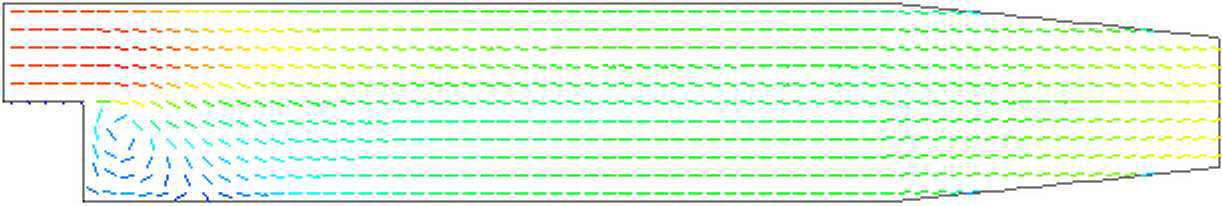
\includegraphics[scale=0.45]{fig-3-6-a.png}\par
 \medskip
 (a) $50$反復後の速度ベクトル\par
 \bigskip
 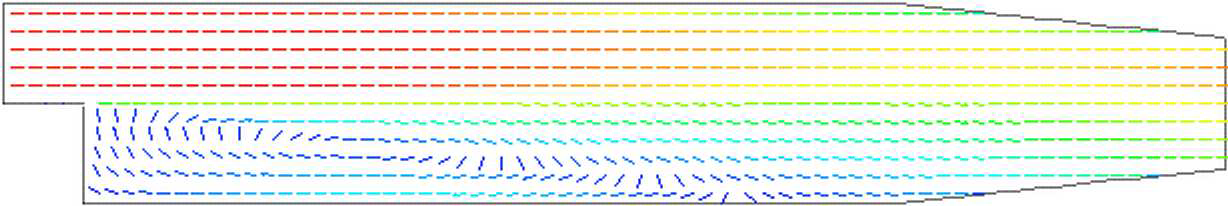
\includegraphics[scale=0.45]{fig-3-6-b}\par
 \medskip
 (b) $1000$反復後の速度ベクトル\par
 \bigskip
 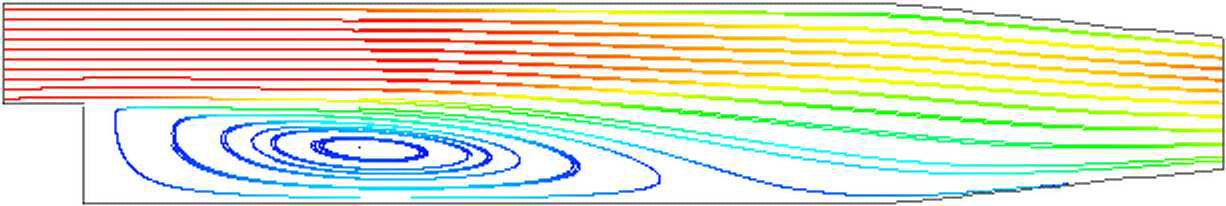
\includegraphics[scale=0.45]{fig-3-6-c}\par
 \medskip
 (c) $1000$反復後の流線\par
 \medskip
 \caption{バック・ステップ内の渦の発達}
 \label{fig:3.6}
\end{figure}



\section{フォワード・ステップ上の超音速流れ}
\label{sec:3.3}
\index{れいだい@例題!フォワード・ステップじょうのちょうおんそくながれ@フォワード・ステップ上の超音速流れ}%
\index{フォワード・ステップじょうのちょうおんそくながれ@フォワード・ステップ上の超音速流れ}%
この例題では前方に面する段差上の超音速流れについて調べます.
問題の概要は,マッハ数$3$の流れが入口付近に段差のある長方形の領域に流入し,
それによって衝撃波を生じるというものです.

この例題では,新たにOpenFOAMの以下のような特徴を紹介します.
\begin{itemize}
 \index{ちょうおんそくながれ@超音速流れ}
 \index{ながれ@流れ!ちょうおんそく@超音速}
 \item 超音速流れ
\end{itemize}


\subsection{問題設定}
\label{ssec:3.3.1}
問題は以下のように定義します.
\begin{description}
 \item[解析領域] 領域は2次元で,\autoref{fig:3.7}に示すように,
            短い入口,それに続いて断面の$20\unit{\%}$の高さの段差があります.


\begin{figure}[ht]
 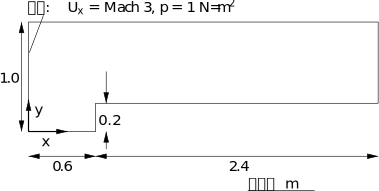
\includegraphics{fig-3-7}
 \caption{フォワード・ステップの計算領域形状}
 \label{fig:3.7}
\end{figure}


 \item[支配方程式] \mbox{}
            \begin{itemize}
             \item 質量保存則
                   \begin{align}
                    \label{eq:3.8}
                    \frac{\partial\rho}{\partial t}
                    + \nabla \inProd (\rho\bm{U}) = 0
                   \end{align}
             \item 理想気体の状態方程式
                   \begin{align}
                    \label{eq:3.9}
                    p = \rho RT
                   \end{align}
             \item ニュートン流体の運動量方程式
                   \begin{align}
                    \label{eq:3.10}
                    \frac{\partial\rho\bm{U}}{\partial t}
                    + \nabla \inProd (\rho\bm{U}\bm{U})
                    - \nabla \inProd \mu\nabla\bm{U}
                    = -\nabla p
                   \end{align}
             \item 流体のエネルギ方程式(いくつかの粘性項は無視),
                   $e = c_{\mathrm{v}}T$であり,
                   フーリエの法則$\bm{q} = -k\nabla T$に基づいています.
                   \begin{align}
                    \label{eq:3.11}
                    \frac{\partial\rho e}{\partial t}
                    + \nabla \inProd (\rho\bm{U}e)
                    - \nabla \inProd \left(\frac{k}{c_{\mathrm{v}}}\right)\nabla e
                    = p\nabla \inProd \bm{U}
                   \end{align}
            \end{itemize}
 \item[初期条件] $U = 0 \unit{m/s}$,$p = 1 \unit{Pa}$,$T = 1 \unit{K}$.
 \item[境界条件] \mbox{}
            \begin{itemize}
             \item 入口(左)は,いずれも\OFboundary{fixedValue}で,
                   速度$\bm{U} = 3 \unit{m/s} = \text{マッハ}3$,
                   圧力$p = 1 \unit{Pa}$および温度$T = 1 \unit{K}$
             \item 出口(右)は,$U$,$p$および$T$,いずれも\OFboundary{zeroGradient}
             \item 滑りなし断熱壁面(下面)
             \item 対称面(上面)
            \end{itemize}
 \item[輸送特性] \mbox{}
            \begin{itemize}
             \item 空気の粘性係数%
\footnote{訳注:原文ではDynamic viscosityとなっているが,
数値・単位からして動粘性係数ではない.}%
                   $\mu = 18.1 \unit{\micro Pa\,s}$
            \end{itemize}
 \item[熱力学特性] \mbox{}
            \begin{itemize}
             \item 定積比熱$c_{\mathrm{v}} = 1.78571 \unit{J/(kg\,K)}$
             \item ガス定数$R = 0.714286 \unit{J/(kg\,K)}$
             \item 熱伝達率$k = 32.3 \unit{\micro W/(m\,K)}$
                   \OFrevision{熱伝達率? 熱伝導率?}
            \end{itemize}
 \item[ケース名] \OFpath{\$FOAM\_TUTORIALS/sonicFoam}%
\footnote{訳注:これは古いバージョンでの配置.
現行バージョンでは\OFpath{\$FOAM\_TUTORIALS/compressible/sonicFoam}にある.}%
            ディレクトリの中にある\OFcase{forwardStep}ケース.
 \item[ソルバ名]
 \index{sonicFoamソルバ@\OFtool{sonicFoam}ソルバ}%
 \index{ソルバ!sonicFoam@\OFtool{sonicFoam}}%
 \OFtool{sonicFoam}: 圧縮性の遷音速・超音速層流%
\footnote{訳注:古いバージョンでは層流のみだったが,現行バージョンでは乱流にも対応している.}%
            の気体の流れの実装.
\end{description}

このケースは,気体中の音速が$c = \sqrt{\gamma RT} = 1 \unit{m/s}$となるように作られています.
その結果,速度がそのままマッハ数となります.例えば,入口の速度$3 \unit{m/s}$はマッハ$3$です.
この音速の計算は,理想気体の関係式$c{\mathrm{p}} - c_{\mathrm{v}} = R$から,
つまり比熱比
\begin{align}
 \label{eq:3.12}
 \gamma = \frac{c_{\mathrm{p}}}{c_{\mathrm{v}}} = \frac{R}{c_{\mathrm{v}}} + 1
\end{align}
から確かめることができます.


\subsection{メッシュ生成}
\label{ssec:3.3.2}
このケースで使うメッシュは比較的単純で,
$x$方向に$0.06 \unit{m}$,$y$方向に$0.05 \unit{m}$の,
一様な長方形セルからなっています.
領域は簡単に三つのブロックに分割され,一つは段差の上面より下側,
あとの二つは段差より上側で,それぞれ段差の前面に対して左側と右側になります.
全ての頂点とブロックを,以下のメッシュ記述ファイルに示します.
\begin{OFverbatim}[file, linenum]
/*--------------------------------*- C++ -*----------------------------------*\
| =========                 |                                                 |
| \\      /  F ield         | OpenFOAM: The Open Source CFD Toolbox           |
|  \\    /   O peration     | Version:  2.2.0                                 |
|   \\  /    A nd           | Web:      www.OpenFOAM.org                      |
|    \\/     M anipulation  |                                                 |
\*---------------------------------------------------------------------------*/
FoamFile
{
    version     2.0;
    format      ascii;
    class       dictionary;
    object      blockMeshDict;
}
// * * * * * * * * * * * * * * * * * * * * * * * * * * * * * * * * * * * * * //

convertToMeters 1;

vertices        
(
    (0 0 -0.05)
    (0.6 0 -0.05)
    (0 0.2 -0.05)
    (0.6 0.2 -0.05)
    (3 0.2 -0.05)
    (0 1 -0.05)
    (0.6 1 -0.05)
    (3 1 -0.05)
    (0 0 0.05)
    (0.6 0 0.05)
    (0 0.2 0.05)
    (0.6 0.2 0.05)
    (3 0.2 0.05)
    (0 1 0.05)
    (0.6 1 0.05)
    (3 1 0.05)
);

blocks          
(
    hex (0 1 3 2 8 9 11 10) (25 10 1) simpleGrading (1 1 1)
    hex (2 3 6 5 10 11 14 13) (25 40 1) simpleGrading (1 1 1)
    hex (3 4 7 6 11 12 15 14) (100 40 1) simpleGrading (1 1 1)
);

edges           
(
);

boundary
(
    inlet
    {
        type patch;
        faces
        (
            (0 8 10 2)
            (2 10 13 5)
        );
    }
    outlet
    {
        type patch;
        faces
        (
            (4 7 15 12)
        );
    }
    bottom
    {
        type symmetryPlane;
        faces
        (
            (0 1 9 8)
        );
    }
    top
    {
        type symmetryPlane;
        faces
        (
            (5 13 14 6)
            (6 14 15 7)
        );
    }
    obstacle
    {
        type patch;
        faces
        (
            (1 3 11 9)
            (3 4 12 11)
        );
    }
);

mergePatchPairs
(
);

// ************************************************************************* //
\end{OFverbatim}


\subsection{ケースの実行}
\label{ssec:3.3.3}
このケースは,$5 \unit{s}$を少し過ぎたあたりで定常状態に達します.
$10 \unit{s}$における圧力の結果を\autoref{fig:3.8}に示します.
この結果からは,段差の根元から生じている圧力の不連続面,つまり衝撃波が顕著に見られます.


\begin{figure}[ht]
 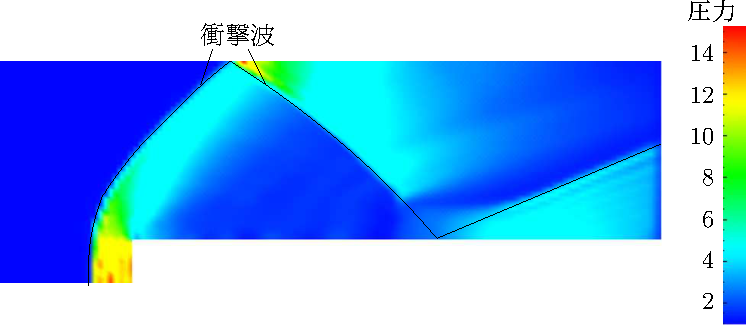
\includegraphics{fig-3-8}
 \caption{フォワード・ステップ問題における衝撃波}
 \label{fig:3.8}
\end{figure}


\subsection{課題}
\label{ssec:3.3.4}
入口の速度を増大させたとき,解に与える影響を調べてみましょう.



\section{加圧された水タンクの減圧}
\index{タンクのげんあつ@タンクの減圧}%
\index{れいだい@例題!タンクのげんあつ@タンクの減圧}%
\label{sec:3.4}
この例題では,加圧した液体で満たされたタンク近くのバルブを急に開くという問題について調べます.
このような問題の結果には圧力波の伝播が重要であり,したがって圧縮性の液体としてモデル化する必要があります.

この例題では,新たにOpenFOAMの以下のような特徴を紹介します.
\begin{itemize}
 \item メッシュの改善
 \index{メッシュ!かいぜん@改善}%
 \item 液体中の圧力波
 \index{あつりょくは@圧力波!えきたいちゅうの@液体中の}
\end{itemize}


\subsection{問題設定}
\label{ssec:3.4.1}
\begin{description}
 \item[解析領域] 領域は2次元で,\autoref{fig:3.9}に示すように,
            小さい流出管路が付いたタンクからなります.


\begin{figure}[ht]
 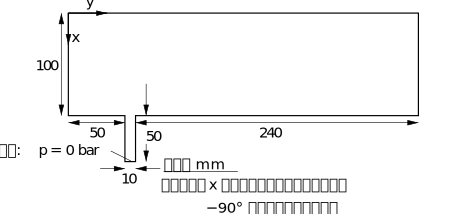
\includegraphics{fig-3-9}
 \caption{流出管路付きタンクの計算領域形状}
 \label{fig:3.9}
\end{figure}


 \item[支配方程式] この問題では,有限の速度で伝播する波を解くために,
            流体の圧縮率$\psi$が必要となります.
            密度$\rho$と圧力$p$を$\psi$と結びつけるには順圧の関係が使われます.
            \begin{itemize}
             \item 質量保存則
                   \begin{align}
                    \label{eq:3.13}
                    \frac{\partial\rho}{\partial t}
                    + \nabla \inProd (\rho\bm{U}) = 0
                   \end{align}
             \item 順圧の関係
                   \begin{align}
                    \label{eq:3.14}
                    \frac{\partial\rho}{\partial p}
                    = \frac{\rho}{K} = \psi
                   \end{align}
                   ここで$K$は体積弾性率です.
             \item \autoref{eq:3.14}は以下のように線形化されます.
                   \begin{align}
                    \label{eq:3.15}
                    \rho \approx \rho_{0} + \psi (p - p_{0})
                   \end{align}
                   ここで$\rho_{0}$と$p_{0}$はそれぞれ参照密度と圧力で,
                   $\rho(p_{0}) = \rho_{0}$です.
             \item ニュートン流体の運動量方程式
                   \begin{align}
                    \label{eq:3.16}
                    \frac{\partial\rho\bm{U}}{\partial t}
                    + \nabla \inProd (\rho\bm{U}\bm{U})
                    - \nabla \inProd \mu\nabla\bm{U}
                    = -\nabla p
                   \end{align}
            \end{itemize}
 \item[境界条件] \OFtool{FoamX}を使って,以下のような物理境界条件を設定できます.
            \begin{itemize}
             \item \OFkeyword{outerWall}は
\index{wall@\OFboundary{wall}!きょうかいじょうけん@境界条件}%
\index{きょうかいじょうけん@境界条件!wall@\OFboundary{wall}}%
				   \OFboundary{wall}条件として指定
             \item \OFkeyword{axis}は
\index{symmetryPlane@\OFboundary{symmetryPlane}!きょうかいじょうけん@境界条件}%
\index{きょうかいじょうけん@境界条件!symmetryPlane@\OFboundary{symmetryPlane}}%
				   \OFboundary{symmetryPlane}として指定
             \item \OFkeyword{nozzle}は$p = 0 \unit{bar}$の
\index{pressureOutlet@\OFboundary{pressureOutlet}!きょうかいじょうけん@境界条件}%
\index{きょうかいじょうけん@境界条件!pressureOutlet@\OFboundary{pressureOutlet}}%
                   \OFboundary{pressureOutlet}として指定
             \item \OFkeyword{front}および\OFkeyword{back}境界は
\index{empty@\OFboundary{empty}!きょうかいじょうけん@境界条件}%
\index{きょうかいじょうけん@境界条件!empty@\OFboundary{empty}}%
                   \OFboundary{empty}として指定
            \end{itemize}
 \item[初期条件] $\bm{U} = \bm{0} \unit{m/s}$,$p = 100 \unit{bar}$.
 \item[輸送特性] \mbox{}
            \begin{itemize}
             \item 水の粘性係数%
\footnote{訳注:原文ではDynamic viscosityとなっているが,
数値・単位からして動粘性係数ではない.}%
                   $\mu = 1.0 \unit{mPa\,s}$
            \end{itemize}
 \item[熱力学特性] \mbox{}
            \begin{itemize}
             \item 水の密度$\rho = 1000 \unit{kg/m^{3}}$
             \item 参照圧力$p_{0} = 1 \unit{bar}$
             \item 水の圧縮率$\psi = 4.54 \times 10^{-7} \unit{s^{2}/m^{2}}$
            \end{itemize}
 \item[ソルバ名]
\index{ソルバ!sonicLiquidFoam@\OFtool{sonicLiquidFoam}}%
\index{sonicLiquidFoamソルバ@\OFtool{sonicLiquidFoam}ソルバ}%
 \OFtool{sonicLiquidFoam}: 遷音速・超音速の圧縮性液体の層流コード.
 \item[ケース名] \OFpath{\$FOAM\_TUTORIALS/sonicLiquidFoam}%
\footnote{訳注:これは古いバージョンでの配置.
現行バージョンでは\OFpath{\$FOAM\_TUTORIALS/compressible/sonicLiquidFoam}にある.}%
            ディレクトリの中にある\OFcase{decompressionTank}ケース.
\end{description}


\subsection{メッシュ生成}
\label{ssec:3.4.2}
% このケースで使うメッシュは比較的単純で,
% $x$方向に$0.06 \unit{m}$,$y$方向に$0.05 \unit{m}$の,
% 一様な長方形セルからなっています.
% 領域は簡単に三つのブロックに分割され,一つは段差の上面より下側,
% あとの二つは段差より上側で,それぞれ段差の前面に対して左側と右側になります.
このケースでモデル化されている形状の
全ての頂点とブロックを,以下のメッシュ記述ファイルに示します.
\begin{OFverbatim}[file, linenum]
/*--------------------------------*- C++ -*----------------------------------*\
| =========                 |                                                 |
| \\      /  F ield         | OpenFOAM: The Open Source CFD Toolbox           |
|  \\    /   O peration     | Version:  2.2.0                                 |
|   \\  /    A nd           | Web:      www.OpenFOAM.org                      |
|    \\/     M anipulation  |                                                 |
\*---------------------------------------------------------------------------*/
FoamFile
{
    version     2.0;
    format      ascii;
    class       dictionary;
    object      blockMeshDict;
}
// * * * * * * * * * * * * * * * * * * * * * * * * * * * * * * * * * * * * * //

convertToMeters 0.1;

vertices        
(
    (0 0 -0.1)
    (1 0 -0.1)
    (0 0.5 -0.1)
    (1 0.5 -0.1)
    (1.5 0.5 -0.1)
    (0 0.6 -0.1)
    (1 0.6 -0.1)
    (1.5 0.6 -0.1)
    (0 3 -0.1)
    (1 3 -0.1)
    (0 0 0.1)
    (1 0 0.1)
    (0 0.5 0.1)
    (1 0.5 0.1)
    (1.5 0.5 0.1)
    (0 0.6 0.1)
    (1 0.6 0.1)
    (1.5 0.6 0.1)
    (0 3 0.1)
    (1 3 0.1)
);

blocks          
(
    hex (0 1 3 2 10 11 13 12) (30 20 1) simpleGrading (1 1 1)
    hex (2 3 6 5 12 13 16 15) (30 5 1) simpleGrading (1 1 1)
    hex (3 4 7 6 13 14 17 16) (25 5 1) simpleGrading (1 1 1)
    hex (5 6 9 8 15 16 19 18) (30 95 1) simpleGrading (1 1 1)
);

edges           
(
);

boundary
(
    outerWall
    {
        type wall;
        faces
        (
            (0 1 11 10)
            (1 3 13 11)
            (3 4 14 13)
            (7 6 16 17)
            (6 9 19 16)
            (9 8 18 19)
        );
    }
    axis
    {
        type symmetryPlane;
        faces
        (
            (0 10 12 2)
            (2 12 15 5)
            (5 15 18 8)
        );
    }
    nozzle
    {
        type patch;
        faces
        (
            (4 7 17 14)
        );
    }
    back
    {
        type empty;
        faces
        (
            (0 2 3 1)
            (2 5 6 3)
            (3 6 7 4)
            (5 8 9 6)
        );
    }
    front
    {
        type empty;
        faces
        (
            (10 11 13 12)
            (12 13 16 15)
            (13 14 17 16)
            (15 16 19 18)
        );
    }
);

mergePatchPairs
(
);

// ************************************************************************* //
\end{OFverbatim}
数値の精度向上のため,圧力場の基準値として$1\unit{bar}$を使います.
内部領域および境界条件のいずれにも,この基準値が上乗せされることに注意してください.


\subsection{実行の準備}
\label{ssec:3.4.3}
計算の設定を始める前に,捉えようとしている現象に対する代表速度を考える必要があります.
いま考えている問題では,流体の速度は非常に小さくなりますが,圧力波は水中の音速で伝播します.
音速は以下のように計算されます.
\begin{align}
 \label{eq:3.17}
 c = \sqrt{\frac{1}{\psi}}
 = \sqrt{\frac{1}{4.54 \times 10^{-7}}}
 = 1483.2 \unit{m/s}
\end{align}
前述のメッシュにおいて,メッシュの代表長さはおよそ$2 \unit{mm}$
(ファイル\OFdictionary{blockMeshDict}で拡大率を$0.1$としたことに注意) です.
\begin{align}
 \label{eq:3.18}
 \nCo = \frac{U\Delta t}{\Delta x}
\end{align}
を使って適切な時間ステップを考えると,およそ$\Delta t = 5 \times 10^{-7} \unit{s}$とすれば
音速に対してクーラン数が$0.35$となります.
コードから出力される(移流速度に基づく)クーラン数は,
2桁ほど小さい値になることにも注意してください.
興味があるのは圧力波の伝播なので,シミュレーション時間を$0.25 \unit{ms}$とします.%
\footnote{訳注:誤植か? 引用されている\OFdictionary{controlDict}では
$0.1 \unit{ms}$になっている.}%
参考に,ファイル
\index{controlDict@\OFdictionary{controlDict}}%
\OFdictionary{controlDict}を以下に引用します.
\begin{OFverbatim}[file, linenum]
/*--------------------------------*- C++ -*----------------------------------*\
| =========                 |                                                 |
| \\      /  F ield         | OpenFOAM: The Open Source CFD Toolbox           |
|  \\    /   O peration     | Version:  2.2.0                                 |
|   \\  /    A nd           | Web:      www.OpenFOAM.org                      |
|    \\/     M anipulation  |                                                 |
\*---------------------------------------------------------------------------*/
FoamFile
{
    version     2.0;
    format      ascii;
    class       dictionary;
    location    "system";
    object      controlDict;
}
// * * * * * * * * * * * * * * * * * * * * * * * * * * * * * * * * * * * * * //

application     sonicLiquidFoam;

startFrom       startTime;

startTime       0;

stopAt          endTime;

endTime         0.0001;

deltaT          5e-07;

writeControl    timeStep;

writeInterval   20;

purgeWrite      0;

writeFormat     ascii;

writePrecision  6;

writeCompression off;

timeFormat      general;

timePrecision   6;

runTimeModifiable true;


// ************************************************************************* //
\end{OFverbatim}


\subsection{ケースの実行}
\label{ssec:3.4.4}


\begin{figure}[ht]
 \tabcolsep=1pt
 \begin{tabular}{lll}
  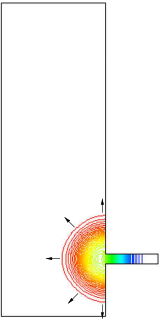
\includegraphics{fig-3-10-a} &
  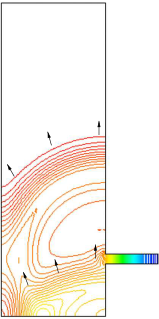
\includegraphics{fig-3-10-b} &
  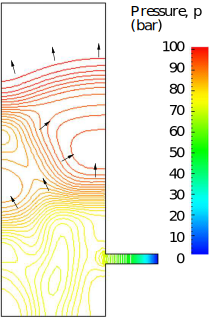
\includegraphics{fig-3-10-c} \\
  (a) $t =  50 \unit{\micro s}$のとき &
  (b) $t = 100 \unit{\micro s}$のとき &
  (c) $t = 150 \unit{\micro s}$のとき
 \end{tabular}
 \caption{圧力波の伝播}
 \label{fig:3.10}
\end{figure}


\OFtool{dxFoam}%
\footnote{訳注:OpenDXを利用したポスト処理ツール.現行バージョンには含まれていない.}%
でケースを実行し,結果を可視化することができます.
液体がノズルから流出していくとともに,ノズルに沿って圧力波が移動していきます.
この圧力波がタンク入口に達すると,その一部はタンク内に伝わっていき,一部は反射されます.
入口パイプの上下で波が反射されることにより,波はタンク内に広がり,伝播していきます.
\autoref{fig:3.10}に圧力を等圧線で示していますので,
\OFrevision{意味不明}%
通常の等値線プロットよりも,波面がよりはっきりと見てとれます.

もしシミュレーションを十分長い時間実行して反射された波がパイプまで帰ってきたら,
負の絶対圧が観測できるでしょう.
このことやその他いくつかの物理原則を表現できるのは,
液体が張力,すなわち負圧を表現できるようにモデリングされているからです.
しかしながら現実には,低圧により液体中の不純物や溶解気体に起因して,
キャビテーションや蒸発・沸騰が起こります.
したがって,実用上,液体の蒸気圧より低い圧力は,
少なくともキャビテーションのプロセスが始まるほど長時間に渡るのでなければ,
一般には無視します.


\subsection{メッシュの改良による解の改善}
\label{ssec:3.4.5}
得られた圧力場の時間発展を見ていると,
圧力波がタンク内に伝播して内壁面で数値的に反射している様子が明らかに見てとれます.
また,いくつものセルを通貨する間に圧力波が鈍っていることも明らかです.
そこで,もっとシャープな波面の解像度を得るために,
メッシュを改良し,時間ステップを短くしてみましょう.
単純に\OFdictionary{blockMeshDict}を編集し,
$x$および$y$方向についてセル数を4倍に増やします.
つまり,ブロック0は \texttt{(30 20 1)} から \texttt{(120 80 1)} とします.
ほかも同様です.
このファイルを使って\OFtool{blockMesh}を実行します.
これに加えて,クーラン数を$1$以下に保つために,
したがって$\Delta t = 10^{-7} \unit{s}$に,時間ステップを短縮する必要があります.
この2度目のシミュレーションは,\autoref{fig:3.11}に示すように,
圧力波の解像度がずいぶん改善しています.


\begin{figure}[ht]
 \tabcolsep=1pt
 \begin{tabular}{lll}
  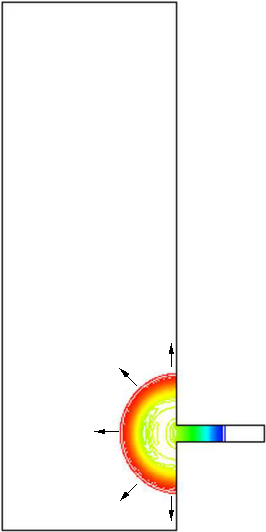
\includegraphics{fig-3-11-a} &
  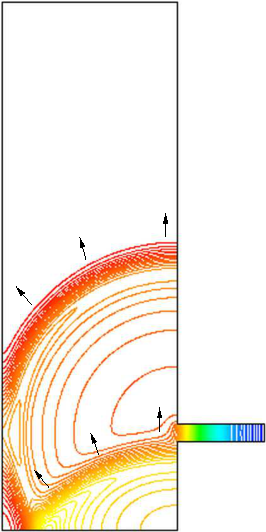
\includegraphics{fig-3-11-b} &
  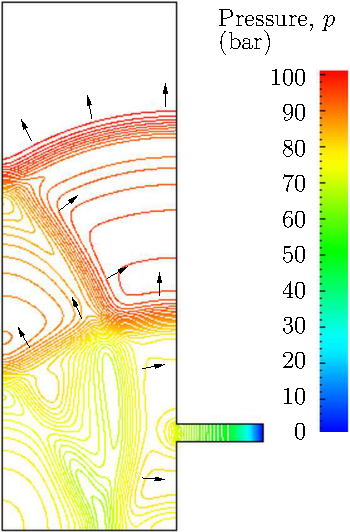
\includegraphics{fig-3-11-c} \\
  (a) $t =  50 \unit{\micro s}$のとき &
  (b) $t = 100 \unit{\micro s}$のとき &
  (c) $t = 150 \unit{\micro s}$のとき
 \end{tabular}
 \caption{改良版メッシュにおける圧力波の伝播}
 \label{fig:3.11}
\end{figure}



\section{磁性液体流れ}
\label{sec:3.5}
この例題では,磁場の中を通過し,
\index{えきたい@液体!でんきのでんどう@電気の伝導}%
電気の伝導を伴う液体の流れについて調べます.
この問題は,
\index{でんじりゅうたいりきがく@電磁流体力学}%
電磁流体力学 (MHD) として知られる,流体力学の一つの分野であり,
\index{ソルバ!mhdFoam@\OFtool{mhdFoam}}%
\index{mhdFoamソルバ@\OFtool{mhdFoam}ソルバ}%
\OFtool{mhdFoam}を使います.


\subsection{問題設定}
\label{ssec:3.5.1}
この問題は
index{れいだい@例題!ハルトマンもんだい@ハルトマン問題}%
ハルトマン問題として知られており,
解析解によって\OFtool{mhdFoam}を検証できるので選びました.
問題は以下のように定義されます.
\begin{description}
 \item[解析領域] 領域は2次元で,\autoref{fig:3.12}に示すように,
            2枚の平行な板に沿った流れからなります.


\begin{figure}[ht]
 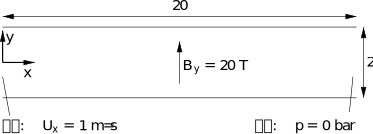
\includegraphics{fig-3-12}
 \caption{ハルトマン問題の計算領域形状}
 \label{fig:3.12}
\end{figure}


 \item[支配方程式] \mbox{}
            \begin{itemize}
             \item 非圧縮性流体の質量保存則
                   \begin{align}
                    \label{eq:3.19}
                    \nabla \inProd \bm{U} = 0
                   \end{align}
             \item 非圧縮性流体の運動量方程式
                   \begin{align}
                    \label{eq:3.20}
                    \frac{\partial\bm{U}}{\partial t}
                    + \nabla \inProd (\bm{U}\bm{U})
                    + \nabla \inProd (2\bm{B}\varGamma_{\bm{BU}}\bm{B})
                    + \nabla \inProd (\nu\bm{U})
                    + \nabla (\varGamma_{\bm{BU}}\bm{B} \biInProd \bm{B})
                    = -\nabla p
                   \end{align}
                   ここで$\bm{B}$は磁束密度であり,
                   $\varGamma_{\bm{BU}} = (2\mu\rho)^{-1}$です.
             \item マクスウェルの方程式
                   \begin{align}
                    \label{eq:3.21}
                    \nabla \times \bm{E} = -\frac{\partial\bm{B}}{\partial t}
                   \end{align}
                   ここで$\bm{E}$は電場強度です.
                   \begin{align}
                    \label{eq:3.22}
                    \nabla \times \bm{B} = 0
                   \end{align}
                   \begin{align}
                    \label{eq:3.23}
                    \nabla \times \bm{H}
                    = \bm{J} + \frac{\partial\bm{D}}{\partial t}
                    = \bm{J}
                   \end{align}
                   $\partial\bm{D}/\partial t \ll \bm{J}$と仮定しています.
                   ここで,$\bm{H}$は磁場強度,$\bm{J}$は電流密度,
                   そして$\bm{D}$は電束密度です.
             \item 電荷の保存則
                   \begin{align}
                    \label{eq:3.24}
                    \nabla \inProd \bm{J} = 0
                   \end{align}
             \item 構成則
                   \begin{align}
                    \label{eq:3.25}
                    \bm{B} = \mu\bm{H}
                   \end{align}
             \item オームの法則
                   \begin{align}
                    \label{eq:3.26}
                    \bm{J} = \sigma(\bm{E} + \bm{U} \times \bm{B})
                   \end{align}
             \item \autoref{eq:3.21},\autoref{eq:3.23},\autoref{eq:3.26}を組み合わせて,
                   回転をとったもの
                   \begin{align}
                    \label{eq:3.27}
                    \frac{\partial\bm{B}}{\partial t}
                    + \nabla \inProd (\bm{U}\bm{B})
                    - \nabla \inProd (\phi_{\bm{B}})
                    - \nabla \inProd (\varGamma_{\bm{B}}\bm{B}) = 0
                   \end{align}
            \end{itemize}
            \item[境界条件] \mbox{}
            \begin{itemize}
             \item \OFkeyword{inlet}は速度固定$\bm{U} = (0,\ 0,\ 0) \unit{m/s}$の
\index{inlet@\OFboundary{inlet}!きょうかいじょうけん@境界条件}%
\index{きょうかいじょうけん@境界条件!inlet@\OFboundary{inlet}}%
                   \OFboundary{inlet}条件として指定%
\footnotemark
             \item \OFkeyword{outlet}は圧力固定$p = 0 \unit{Pa}$の
\index{outlet@\OFkeyword{outlet}!きょうかいじょうけん@境界条件}%
\index{きょうかいじょうけん@境界条件!outlet@\OFkeyword{outlet}}%
                   \OFboundary{outlet}として指定
\addtocounter{footnote}{-1}
\footnote{訳注:古いバージョンでは\OFboundary{inlet},
\OFboundary{outlet}という境界条件があった?(未確認)
現行バージョンでは,それぞれ\OFkeyword{U}あるいは\OFkeyword{p}を\OFboundary{fixedValue}とし,
他方を\OFboundary{zeroGradient}とする.}%
             \item \OFkeyword{upperWall}は$\bm{B} = (0,\ 20,\ 0) \unit{T}$の
\index{きょうかいじょうけん@境界条件!wall@\OFboundary{wall}}%
\index{wall@\OFboundary{wall}!きょうかいじょうけん@境界条件}%
                   \OFboundary{wall}として指定
             \item \OFkeyword{lowerWall}は$\bm{B} = (0,\ 20,\ 0) \unit{T}$の
                   \OFboundary{wall}として指定
             \item \OFkeyword{front}および\OFkeyword{back}境界は
\index{empty@\OFboundary{empty}!きょうかいじょうけん@境界条件}%
\index{きょうかいじょうけん@境界条件!empty@\OFboundary{empty}}%
                   \OFboundary{empty}として指定
            \end{itemize}
 \item[初期条件] $\bm{U} = \bm{0} \unit{m/s}$,$p = 100 \unit{Pa}$,
            $\bm{B} = (0,\ 20,\ 0) \unit{T}$.
 \item[輸送特性] \mbox{}
            \begin{itemize}
             \item 動粘性係数$\nu = 1 \unit{mPa\,s}$
             \item 密度$\rho = 1 \unit{kg\,m/s}$
             \item 電気伝導率$\sigma = 1 \unit{(\Omega\,m)}$
             \item 透磁率$\mu = 1 \unit{H/m}$
            \end{itemize}
 \item[ソルバ名]
\index{mhdFoamソルバ@\OFtool{mhdFoam}ソルバ}%
\index{ソルバ!mhdFoam@\OFtool{mhdFoam}}%
 \OFtool{mhdFoam}: 非圧縮性で層流の電磁流体コード
 \item[ケース名] \OFpath{\$FOAM\_TUTORIALS/mhdFoam}%
\footnote{訳注:これは古いバージョンでの配置.
現行バージョンでは\OFpath{\$FOAM\_TUTORIALS/electromagnetics/mhdFoam}にある.}%
            ディレクトリの中にある\OFcase{hartmann}ケース.
\end{description}


\subsection{メッシュ生成}
\label{ssec:3.5.2}
計算領域は$x$方向に$100$セル,$y$方向に$40$セルとして単純にモデル化されています.
頂点およびブロックを以下のメッシュ定義ファイルに示します.
\begin{OFverbatim}[file, linenum]
/*--------------------------------*- C++ -*----------------------------------*\
| =========                 |                                                 |
| \\      /  F ield         | OpenFOAM: The Open Source CFD Toolbox           |
|  \\    /   O peration     | Version:  2.2.0                                 |
|   \\  /    A nd           | Web:      www.OpenFOAM.org                      |
|    \\/     M anipulation  |                                                 |
\*---------------------------------------------------------------------------*/
FoamFile
{
    version     2.0;
    format      ascii;
    class       dictionary;
    object      blockMeshDict;
}
// * * * * * * * * * * * * * * * * * * * * * * * * * * * * * * * * * * * * * //

convertToMeters 1;

vertices        
(
    (0 -1 0)
    (20 -1 0)
    (20 1 0)
    (0 1 0)
    (0 -1 0.1)
    (20 -1 0.1)
    (20 1 0.1)
    (0 1 0.1)
);

blocks          
(
    hex (0 1 2 3 4 5 6 7) (100 40 1) simpleGrading (1 1 1)
);

edges           
(
);

boundary
(
    inlet
    {
        type patch;
        faces
        (
            (0 4 7 3)
        );
    }
    outlet
    {
        type patch;
        faces
        (
            (2 6 5 1)
        );
    }
    lowerWall
    {
        type patch;
        faces
        (
            (1 5 4 0)
        );
    }
    upperWall
    {
        type patch;
        faces
        (
            (3 7 6 2)
        );
    }
    frontAndBack
    {
        type empty;
        faces
        (
            (0 3 2 1)
            (4 5 6 7)
        );
    }
);

mergePatchPairs
(
);

// ************************************************************************* //
\end{OFverbatim}


\subsection{ケースの実行}
\label{ssec:3.5.3}
\OFtool{dxFoam}%
\footnote{訳注:OpenDXを利用したポスト処理ツール.現行バージョンには含まれていない.}%
でケースを実行し,結果を可視化することができます.
$\bm{U}$ベクトル場から個別のスカラ成分を取り出す
\OFtool{Ucomponents}ユーティリティも便利です.
電磁流体の流れは,主として,
粘性力に対する電磁的な体積力の比を表すハルトマン数%
\footnote{訳注:原文では$M$が使われているが,わかりにくいので$\nHa$とした.}%
\begin{align}
 \label{eq:3.28}
 \nHa = BL\sqrt{\frac{\sigma}{\rho\nu}}
\end{align}
によって支配されます.ここで$L$は特性長さです.
このケースでは$B_{y} = 20 \unit{T}$,$\nHa = 20$であり,
粘性力に対して電磁的な体積力が支配的です.
したがって,流れがすっかり定常になった$t = 2 \unit{s}$において,
中央の$x = 10 \unit{m}$に沿った断面でみた速度分布は大部分が平坦になっています.
\OFtool{dxFoam}で$U_{x}$の分布をグラフにプロットすることができます.
さて,磁束密度$\bm{B}$を$1 \unit{T}$に減らして,
計算コードと\OFtool{Ucomponents}を再実行してみましょう.
このケースでは$\nHa = 1$となり,もはや電磁的な体積力が支配的ではなくなります.
したがって,\autoref{fig:3.13}に示すように,
速度分布はポアズイユ流れの特徴である放物線状となります.
コードを検証するために,
\begin{align}
 \label{eq:3.29}
 \frac{U_{x}(y)}{U_{x}(0)}
 = \frac{\cosh\nHa - \cosh\nHa (y/L)}{\cosh\nHa - 1}
\end{align}
で与えられる速度分布$U_{x}$の解析解を\autoref{fig:3.13}に重ねて示します.
ここで,特性長さ$L$は計算領域の幅の半分,つまり$1 \unit{m}$です.


\begin{figure}[ht]
 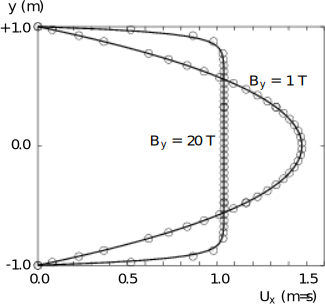
\includegraphics{fig-3-13}
 \caption{$B_{y} = 1 \unit{T}$および$B_{y} = 20 \unit{T}$のハルトマン問題における速度分布}
 \label{fig:3.13}
\end{figure}

